\section{Case Study}
\label{CaseStudy}

	To illustrate the applicability of the proposed methodology, a case study with real data from the Brazilian power system is presented. For expository purpose, this case study is based on the same business scheme presented in \cite{RobustSpotPrice}. We assume an ETC with an opportunity to sell an one-year supply contract for the year of 2012 with $Q^{\text{sell}} = 10$ avgMW and $P^{\text{sell}} = 140$ \$/MWh with monthly settlements $H = \{1, \dots, 12\}$. Two complementary renewable sources are available to back the short position: (i) a Wind Power (WP) plant with 21.12 avgMW of FEC; and (ii) a run-of-river Small Hydro (SH) plant with 17.4 avgMW of FEC. Both sources agreed to sell 100\% of their firm energy for $P^{\text{res}} = 90$ \$/MWh. The risk aversion parameters are set to $\alpha = $ 0.95 and $\underline{R}^{\text{risk}} = $ 2.32 MM\$

	To obtain the scenario-representation of the spot price uncertainty, a fundamentalist approach based on least cost dispatch was applied to optimize the system's operation \cite{SDDPMathProg}. Official data from December 2011 was used as input for the dispatch model. These scenarios were used to compute the nominal (random) spot price $\accentset{\sim}{\boldsymbol{\pi}}$. With respect to the ambiguity constraints, we assume a deterministic spot price reference $(\pi^{\text{o}}_{t,\omega} \rightarrow \pi^{\text{o}}_{t})$ and maximum/minimum deviation $(\Delta^{\pm}_{t,\omega} \rightarrow \Delta^{\pm}_{t})$ parameters in order to construct the optimal portfolio in a portfolio-oriented stress analysis, similar to \cite{RobustSpotPrice}. Six levels of protection were assumed. The budget level $K$ and the corresponding minimum profit requirement $\underline{R}_{K}^{\text{amb}}$ used in this study are shown in Table \ref{AmbiguityConstraintsParam}. To represent the uncertainty on renewable production, we make use of the methodology presented in \cite{FosteringWPP} to simulate scenarios of wind and hydro generation correlated with the set of nominal spot price scenarios. 2000 correlated scenarios of renewable production and energy spot price were generated for this case study. We refer to Case Study I in \cite{RobustSpotPrice} (Section 5.A) for the statistics of the set of scenarios simulated and the description of parameters used in the robust counterpart.
%
\begin{table}
	\renewcommand{\arraystretch}{1.1}
	\centering
	\caption{Budget Level $K$ and Minimum Profit Requirement $\underline{R}_{K}^{\text{amb}}$ (MM\$)}
	\begin{tabular}{ r | c  c  c  c  c  c }
		$ \boldsymbol{K} $ & 0.5 & 1.0 & 1.5 & 2.0 & 2.5 & 3.0 \\
		\hline
		$ \underline{\boldsymbol{R}}_{K}^{\text{amb}}$ & 2.0 & 0.6 & -0.8 & -2.2 & -3.4 & -4.7
	\end{tabular}
	\label{AmbiguityConstraintsParam}
\end{table}

	To hedge the business, we assume available a single call option in each month with $Q_{j}^{\text{call}} = $ 10 avgMW. In Table \ref{Table_CallPriceStrike}, the strike price (columns two and six) and premium (columns three and seven) of each option is presented. The strike price was set to the monthly average of the spot price simulation and the corresponding premium was defined such that the expected revenue of the option is null: $\mathbb{E} \big[\accentset{\sim}{R}_{j}^{\text{call}}\big] = 0 \implies P_{j}^{\text{call}} = \mathbb{E}[ \max\{0, \accentset{\sim}{\pi_{t}} - \Gamma_{j}^{\text{call}}\}]$. 

	Three different cases were considered: 
\begin{itemize}
	\item[C1:] the classical model with only the risk constraint and without call options $(\mathcal{K} = \emptyset$ and $C_{t} = \emptyset, \forall ~ t \in H)$; 
	\item[C2:] a model with both risk and ambiguity constraints, but without call options $(C_{t} = \emptyset, \forall ~ t \in H)$; 
	\item[C3:] a model with risk and ambiguity constraints and call options. 
\end{itemize}

	Each model was solved in less than a minute in a Dell Inspiron 15R Special Edition Laptop. The optimal amount sold in the supply contract and bought from each renewable source are shown in columns two to four of Table \ref{ContractingStrat}. In case C3, the optimal portfolio of call options is presented in columns four and eight of Table \ref{Table_CallPriceStrike}. Note that in all cases, the optimal strategy is to sell the whole supply contract. However, in C1 and C2, an excess of renewable energy is bought to help mitigate the price and quantity risk. Particularly in C2, such hedge exceeds 7\% of the supply contract due to the action of the ambiguity constraints on the portfolio. Specifically, the optimization model must find a renewable portfolio that guarantees a feasible worst-case revenue for the different levels of ambiguity; and this is achieved by reducing the exposure of the ETC to energy deficits, which can be translated into the combination of an increase on the total level of renewable energy bought with a flatter production of the renewable portfolio, i.e. the purchase of more hydro to complement the wind.
%
\begin{table}
	\renewcommand{\arraystretch}{1.2}
	\centering
	\caption{Parameters and Optimal Portfolio (avgMW) of Call Options}
	\begin{tabular}{ l | c  c  c || l | c  c  c }
		& $\boldsymbol{\Gamma}_{j}^{\text{call}}$ & $\boldsymbol{P}_{j}^{\text{call}}$ & $\boldsymbol{Q}_{j}^{*}$ &  & $\boldsymbol{\Gamma}_{j}^{\text{call}}$ & $\boldsymbol{P}_{j}^{\text{call}}$ & $\boldsymbol{Q}_{j}^{*}$ \\
		\hline
		\textbf{Jan.} & \textcolor{white}{0}45 & 15.00 & 6.86 & \textbf{Jul.} & \textcolor{white}{0}80 & 34.14 & 2.11 \\
		\textbf{Feb.} & \textcolor{white}{0}55 & 21.78 & 6.37 & \textbf{Aug.} & \textcolor{white}{0}80 & 34.50 & 1.27 \\
		\textbf{Mar.} & \textcolor{white}{0}60 & 25.48 & 9.79 & \textbf{Sept.} & \textcolor{white}{0}90 & 38.66 & 2.09 \\ 
		\textbf{Apr.} & \textcolor{white}{0}70 & 27.04 & 9.99 & \textbf{Oct.} & 100 & 44.02 & 0.19\\ 
		\textbf{May} & \textcolor{white}{0}70 & 30.40 & 9.94 & \textbf{Nov.} & 105 & 46.64 & 0.20 \\
		\textbf{Jun.} & \textcolor{white}{0}75 & 31.58 & 1.58 & \textbf{Dec.} & \textcolor{white}{0}95 & 45.25 & 1.10
	\end{tabular}
	\label{Table_CallPriceStrike}
\end{table}
%
\begin{table}
	\renewcommand{\arraystretch}{1.0}
	\centering
	\caption{Optimal Mix of Supply Contract/Renewable Sources (avgMW) and Back Test (MM\$)}
	\begin{tabular}{ r | c  c  c | c || c  c  c }
%		& & & & & \multicolumn{3}{c}{\textbf{Back Test}} \\
		& \textbf{WP} & \textbf{SH} & \textbf{Supply} & \textbf{Excess} & \textbf{2008} & \textbf{2010} & \textbf{2012} \\
		\hline
		\textbf{C1} & 9.85 & 0.18 & 10.00 & 0.04 & 3.22 & 6.06 & 6.01 \\
		\textbf{C2} & 8.09 & 2.65 & 10.00 & 0.74 & 3.79 & 5.55 & 6.30 \\
		\textbf{C3} & 10.00 & 0.00 & 10.00 & 0.00 & 5.75 & 5.23 & 7.59
	\end{tabular}
	\label{ContractingStrat}
\end{table}

	An interesting result occurs in case C3. The optimal portfolio of renewable sources is composed only by the WP plant. In addition, no excess of energy is bought. One way to interpret this result is to observe that the spot price dynamics over time is similar to the wind power production one. More specifically, periods of high spot prices (typically occurring in the last months of the year) are likely to be coincident with periods of high wind production and vice-versa. In contrast, small hydro generation has a complementary dynamics with respect to these two sources. Therefore, although the SH can be used to reduce the short-term exposure of the WP in periods of energy deficit and high spot price, this hedge is stochastic once the production of the SH is uncertain. In this sense, call options posses a significant advantage since they provide ``deterministic'' hedge against energy deficit and high spot price. Thus, the (uncertain) SH generation loses all its value in the portfolio in the presence of call options. Finally, observe that the amount of energy acquired from the call options in the first five months of the year is significantly higher than the amount bought in rest of the year, covering exactly the period of high probability of low wind production. This result is in accordance to the hedge function that the options have in the portfolio. To corroborate this conclusion, Fig. \ref{IAF_CVaR} shows the inverse accumulated probability function restricted to the 5\% worst-scenarios of the business revenue under the nominal scenarios of spot price. Note that the distribution of C3 dominates the other cases, which reveals the benefits in risk mitigation that the combination of call options hedge within an ambiguity-constraint framework provide. Additionally, when a comparison is made on the worst-case revenue, these benefits are notorious. Table \ref{InSample_Analysis} presents the expected value of the nominal revenue and $\text{CVaR}_{0.95}$ of the worst-case revenue under the different protection levels $\mathcal{K}$. Observe that the performance of the with the inclusion of the set of ambiguity constraints (C2) is better than the classical case (C1) in a worst-case analysis (columns three-eight of Table \ref{InSample_Analysis}), but worst in profit expectation (second column), as expected. However, when the set of call options are available to compose the ETC portfolio (C3), both the performance of the worst-case case and nominal revenues are significantly better with respect to C1 and C2 and even positive for all cases of $K \in \mathcal{K}$. 
%
\begin{figure}[!t]
	\centering
	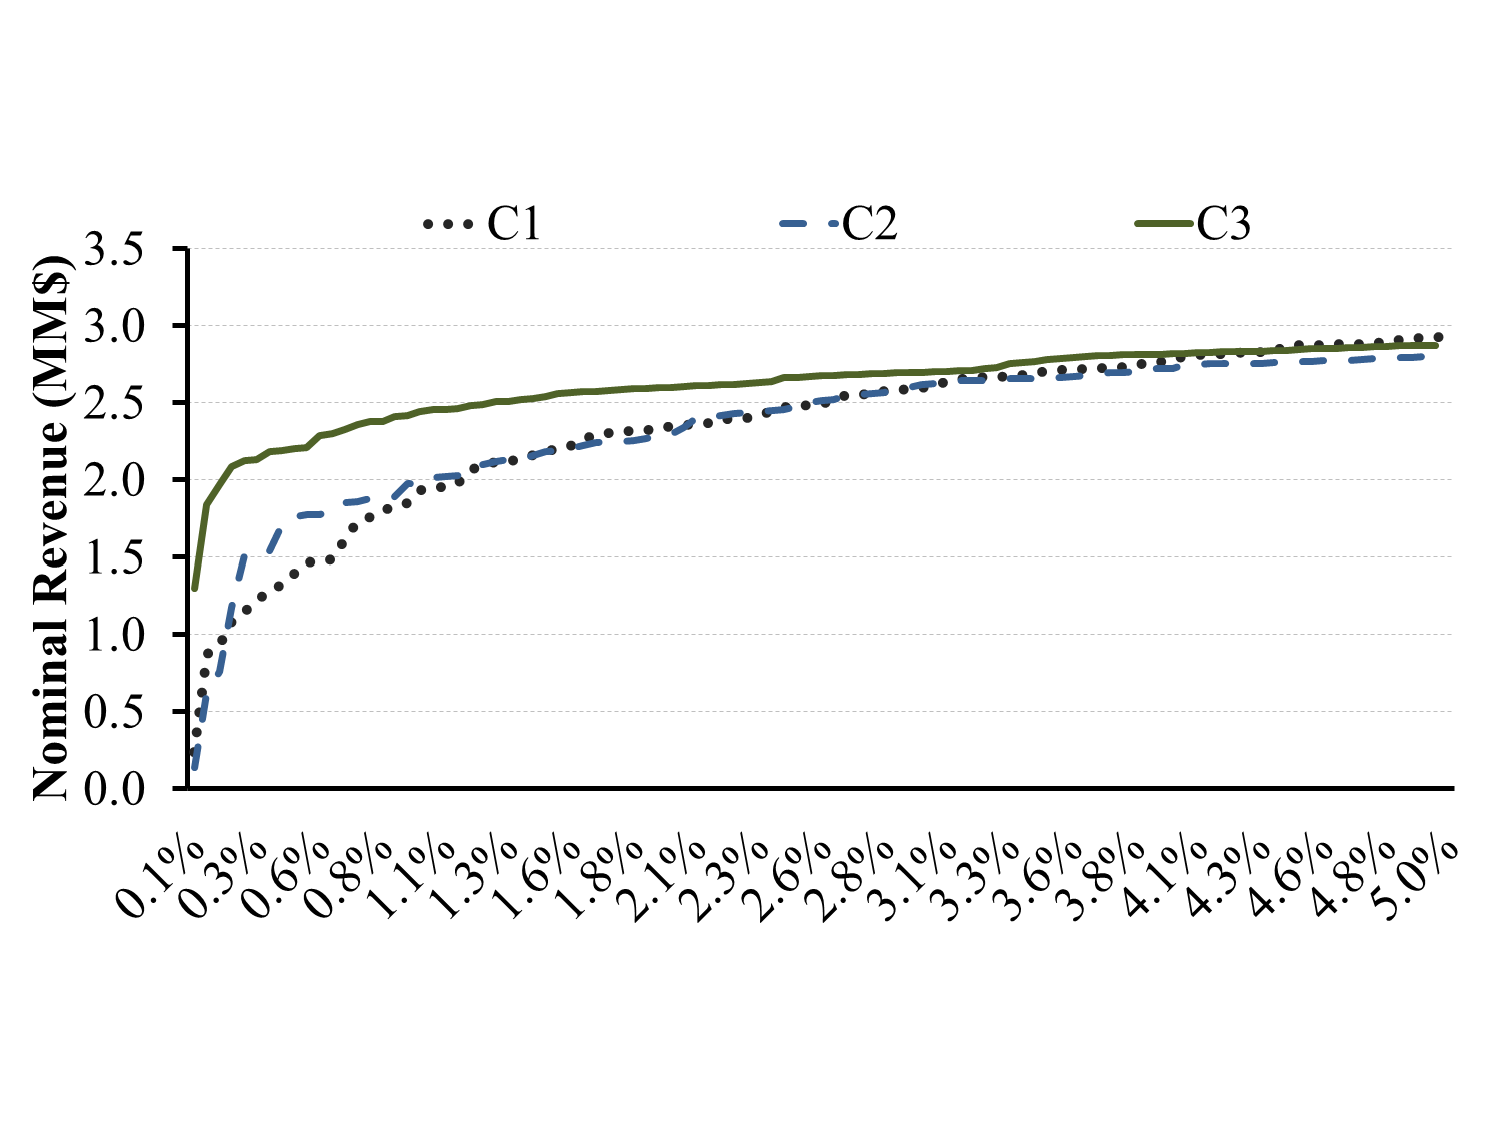
\includegraphics[viewport= 14 98 701 443, clip, width=0.45\textwidth]{./Figures/CurvaPertinencia.pdf}
	\caption{Inverse accumulate probability function restricted to the 5\% worst scenarios of the nominal revenue for the three cases.}
	\label{IAF_CVaR}
\end{figure}
%
\begin{table}
	\renewcommand{\arraystretch}{1.2}
	\centering
	\caption{Expected value of the nominal revenue and $\text{CVaR}_{0.95}$ of the worst-case revenue (MM\$). * identifies a bind constraint.}
	\begin{tabular}{ r | c || c  c  c  c  c  c }
		& & \multicolumn{6}{c}{$\boldsymbol{\text{CVaR}_{0.95}}$} \\
		& $\boldsymbol{\mathbb{E}[\accentset{\sim}{R}]}$ & $\boldsymbol{\accentset{\sim}{R}_{0.5}^{\text{WC}}}$ & $\boldsymbol{\accentset{\sim}{R}_{1.0}^{\text{WC}}}$ & $\boldsymbol{\accentset{\sim}{R}_{1.5}^{\text{WC}}}$ & $\boldsymbol{\accentset{\sim}{R}_{2.0}^{\text{WC}}}$ & $\boldsymbol{\accentset{\sim}{R}_{2.5}^{\text{WC}}}$ & $\boldsymbol{\accentset{\sim}{R}_{3.0}^{\text{WC}}}$ \\
		\hline
		\textbf{C1} & 4.66 & 1.85 & -0.05 & -1.94 & -3.77 & -5.53 & -7.26 \\
		\textbf{C2} & 4.12 & 2.00* & 0.60* & -0.79 & -2.13 & -3.40* & -4.65 \\
		\textbf{C3} & 4.70 & 2.13 & 1.56 & 1.03 & 0.58 & 0.35 & 0.17
	\end{tabular}
	\label{InSample_Analysis}
\end{table}

	In order to validate the proposed methodology, we perform a back test analysis on each of the portfolios against observed data for the uncertain variables. We choose three special years to perform the analysis: (i) 2012, the contract year; (ii) 2010, year where the spot price uncertainty realized as expected (low values in the beginning of the year and high values in the end); (iii) 2008, year in which the observed values of spot price occurred exactly opposite to expected. The financial result of each portfolio in each of the three years is shown in the last three columns of Table \ref{ContractingStrat}. Note that proposed methodology (C2 and C3) outperforms the classical risk-constrained approach (C1) in 2008 and 2012. However, the same performance is not observed in 2010. This result is expected and adequately capture the applicability and relevance of the proposed model with ambiguity treatment. Since the spot price dynamics for 2010 follows a expected pattern, i.e. a pattern explicitly considered in the scenarios used to evaluate the nominal revenue, the classical allocation model (C1) ``optimizes'' the portfolio for the uncertainty environment occurred in 2010. Therefore, the protection imposed by the ambiguity constraints against deviations on the simulated spot scenarios sub-optimizes the portfolio leading to lower gains in 2010. On the other hand, for 2008, a year with observed spot price dynamics different from to the simulated one, the protection created by the ambiguity constraints makes the portfolio allocated by models C2 and C3 to outperform the classical approach C1. Finally, in 2012, we observed atypical spikes in the beginning of the year thus not meeting the expected dynamics of lower prices in this period (bars in Fig. \ref{Backtest_2012}). Therefore, once again, the proposed methodology with ambiguity constraints outperforms the classical one for the same reasons discussed earlier.
%
\begin{figure}[!t]
	\centering
	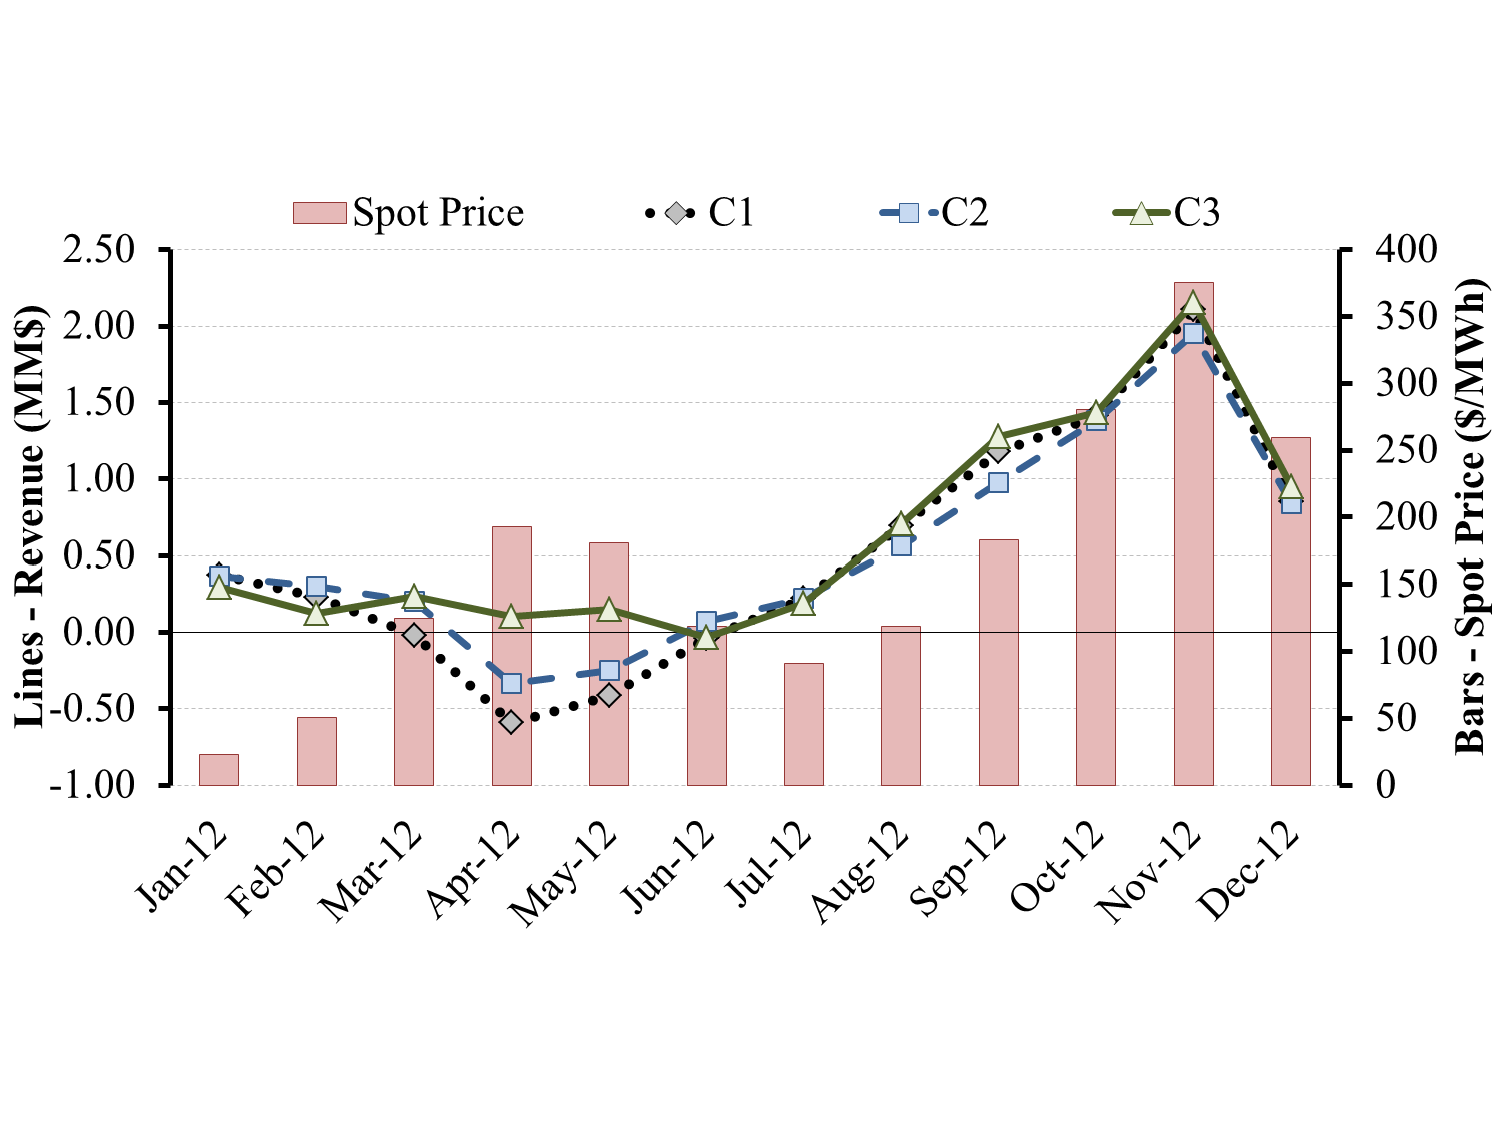
\includegraphics[viewport= 5 95 717 446, clip, width=0.45 \textwidth]{./Figures/BackTest_2012.pdf}
	\caption{Spot prices and revenue profile of the portfolios for the observed data (renewable generation and spot prices) during the contract horizon.}
	\label{Backtest_2012}
\end{figure}

	Finally, to better understand the benefits of the combination of ambiguity constraints and call options, Fig. \ref{Backtest_2012} presents the revenue profile of each portfolio in each month of the contract year. Note that, since the expected pattern of the spot price in the beginning of the years is of low values, without the ambiguity constraints, the set of call options are likely to have no value in the ETC's portfolio. Therefore, if some spikes are observed in this period, as occurred in 2012, the ETC will not be protected. In this context, the ambiguity constraints introduce a robustness in the portfolio allocation that the nominal simulation alone cannot provide. Thus, to protect the portfolio against this ``new'' information, the call options available for the beginning of the year gains value. As a consequence, the revenue of the months of April and May of C3 are strictly positive whereas of C1 and C2 are negative.